\documentclass[aspectratio=169,11pt]{beamer}

\usepackage[T1]{fontenc}
\usepackage{lmodern}
\usepackage{xcolor}
\usepackage{tikz}
\usepackage{booktabs}
\usepackage{array}
\usepackage{listings}
\usepackage{textcomp}

\definecolor{navy}{HTML}{0A2540}
\definecolor{orange}{HTML}{D97706}
\definecolor{green}{HTML}{15803D}
\definecolor{grey}{HTML}{6B7280}
\definecolor{lightgrey}{HTML}{E5E7EB}
\definecolor{red}{HTML}{B91C1C}
\definecolor{codebg}{HTML}{F8FAFC}

\usecolortheme[named=navy]{structure}
\setbeamertemplate{navigation symbols}{}
\setbeamercolor{frametitle}{fg=navy}
\setbeamerfont{frametitle}{series=\bfseries,size=\Large}
\setbeamertemplate{footline}{%
  \vspace{0.3em}%
  \hbox{\hspace{0.9em}\color{grey}\tiny exp27 \textperiodcentered\ iter\_R4\_grow\_05\_10\_15\_25 \textperiodcentered\ MarinFold 1B\hfill\insertframenumber{} / \inserttotalframenumber\hspace{0.9em}}\vspace{0.4em}}
\setbeamertemplate{frametitle}{%
  \vspace*{0.4em}\hspace*{0.6em}\insertframetitle\par
  \vspace*{-0.2em}\hspace*{0.6em}\textcolor{orange}{\rule{0.93\paperwidth}{1.2pt}}\vspace*{-0.4em}
}

\lstdefinestyle{code}{
  basicstyle=\ttfamily\small\color{navy},
  backgroundcolor=\color{codebg},
  frame=single,
  framerule=0.4pt,
  rulecolor=\color{navy},
  numbers=none,
  breaklines=false,
  showstringspaces=false,
  xleftmargin=0.6em,
  xrightmargin=0.6em,
  aboveskip=0.4em,
  belowskip=0.4em,
}

% Inline mono with no rule
\newcommand{\code}[1]{\texttt{\small\color{navy}#1}}

\begin{document}

% --- Slide 1: title ---
\begin{frame}[plain]
  \begin{center}
    \vspace{1.0cm}
    {\Huge\bfseries\ttfamily\color{navy}iter\_R4\_grow\_05\_10\_15\_25}\\[0.6cm]
    {\Large\color{navy}Iterative contact-seeded inference for MarinFold 1B}\\[0.7cm]
    {\large\color{green}\bfseries Lifts mean LDDT on the FoldBench-10 train set from
      0.250 \textrightarrow{} 0.351 \quad (+40.7\%)}\\[1.5cm]
    {\small\color{grey}\ttfamily Issue \#27 \textperiodcentered\ exp27 \textperiodcentered\
      branch exp/27-improved-inference-algorithm}
  \end{center}
\end{frame}

% --- Slide 2: the problem ---
\begin{frame}[fragile]{The problem}
  \begin{itemize}
    \setlength\itemsep{0.4em}
    \item MarinFold 1B is a Llama-arch LLM trained on protein documents in the
          \code{contacts-and-distances-v1} grammar:
  \end{itemize}
  \begin{lstlisting}[style=code]
<begin_sequence> <AAs> <begin_statements>
  [<*-range-contact> <p_i> <p_j>]*
  <distance> <p_i> <p_j> <atom_i> <atom_j>  ->  <d_X.X>
  \end{lstlisting}
  \begin{itemize}
    \setlength\itemsep{0.4em}
    \item \textbf{Baseline readout} (exp20): prompt with \code{<begin\_statements>},
          then for every $(i, j)$ pair read the next-token distribution over
          \code{<d\_X.X>} bins. Zero context, no autoregression, no seeded contacts.
    \item On the 10-protein FoldBench train set: \textbf{mean LDDT = 0.2496}
          (median 0.250, per-protein 0.151--0.449).
    \item \textbf{\color{green}Goal:} clear \textbf{+50\%} over baseline (mean LDDT
          $\geq 0.3744$), within $5\times$ the baseline wall-clock
          ($\leq 6920$\,s on one A100).
  \end{itemize}
\end{frame}

% --- Slide 3: key insight ---
\begin{frame}{Key insight: the model is great with context}
  \begin{center}
    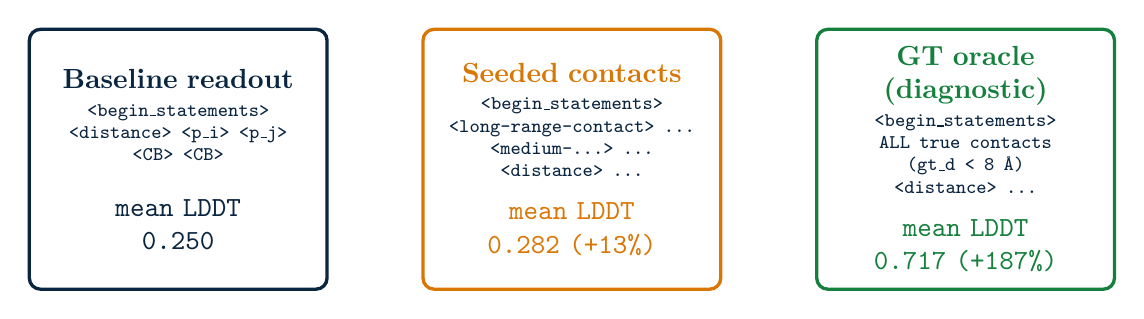
\begin{tikzpicture}[
      box/.style={draw, line width=1.2pt, rounded corners=4pt,
                  text width=3.5cm, align=center, minimum height=3.3cm,
                  inner sep=4pt},
    ]
      \node[box, draw=navy] (base) at (0, 0) {%
        \textbf{\color{navy}Baseline readout}\\[0.2em]
        \scriptsize\ttfamily\color{navy}
        <begin\_statements>\\
        <distance> <p\_i> <p\_j>\\
        <CB> <CB>\\[1.1em]
        \normalsize\color{navy}\bfseries
        mean LDDT\\ 0.250
      };
      \node[box, draw=orange] (seed) at (5, 0) {%
        \textbf{\color{orange}Seeded contacts}\\[0.2em]
        \scriptsize\ttfamily\color{navy}
        <begin\_statements>\\
        <long-range-contact> ...\\
        <medium-...> ...\\
        <distance> ...\\[0.5em]
        \normalsize\color{orange}\bfseries
        mean LDDT\\ 0.282 (+13\%)
      };
      \node[box, draw=green] (orac) at (10, 0) {%
        \textbf{\color{green}GT oracle\\(diagnostic)}\\[0.2em]
        \scriptsize\ttfamily\color{navy}
        <begin\_statements>\\
        ALL true contacts\\
        (gt\_d < 8 \r{A})\\
        <distance> ...\\[0.5em]
        \normalsize\color{green}\bfseries
        mean LDDT\\ 0.717 (+187\%)
      };
    \end{tikzpicture}
  \end{center}
  \vspace{0.4em}
  \begin{center}
    $\rightarrow$ contact-prediction quality is the bottleneck for honest
    algorithms.\\[0.6em]
    {\Large\itshape\color{orange}How do we get honest, high-quality contacts at
      inference time?}\\[0.6em]
    \textbf{Idea:} iterate. The model's distance readout under a seeded prefix is
    sharper\\
    $\rightarrow$ extract NEW high-confidence contacts from the round-$N$
    distogram $\rightarrow$ re-seed.
  \end{center}
\end{frame}

% --- Slide 4: enrichment chart ---
\begin{frame}{Iteration enriches the high-confidence contact pool}
  \begin{center}
    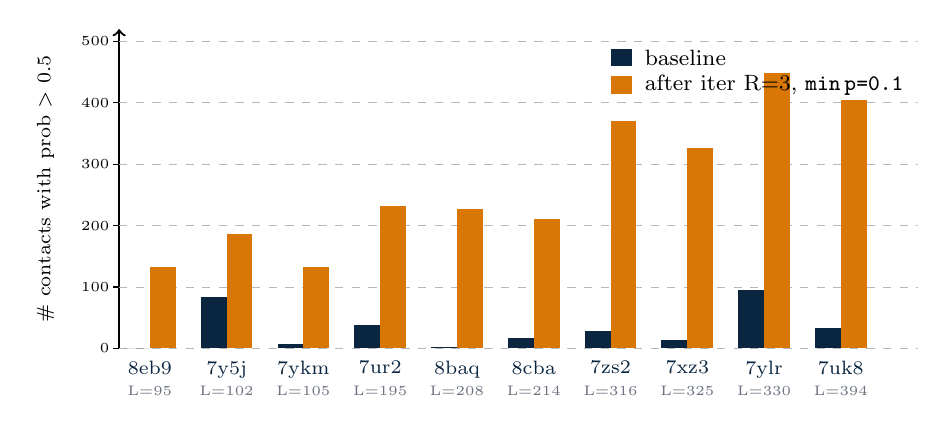
\begin{tikzpicture}[scale=0.78]
      % Y axis with ticks
      \draw[->, thick] (0,0) -- (0,5.2);
      \node[rotate=90, anchor=south, font=\scriptsize] at (-0.9, 2.6)
        {\# contacts with prob $>$ 0.5};
      \foreach \y in {0,100,200,300,400,500} {
        \pgfmathsetmacro\yy{\y/100}
        \draw (-0.1, \yy) -- (0, \yy) node[left, font=\tiny]{\y};
        \draw[grey!50, dashed, very thin] (0, \yy) -- (13, \yy);
      }
      \def\barw{0.42}
      \def\spc{1.25}
      \foreach[count=\i from 0] \name/\Len/\bv/\iv in {%
        8eb9/95/0/132, 7y5j/102/84/186, 7ykm/105/7/132, 7ur2/195/38/232,
        8baq/208/3/227, 8cba/214/17/210, 7zs2/316/28/370, 7xz3/325/13/326,
        7ylr/330/95/449, 7uk8/394/33/404} {
        \fill[navy] (\spc*\i + 0.5 - \barw, 0) rectangle ++(\barw, \bv/100);
        \fill[orange] (\spc*\i + 0.5, 0) rectangle ++(\barw, \iv/100);
        \node[anchor=north, font=\scriptsize, text=navy]
          at (\spc*\i + 0.5, -0.05) {\name};
        \node[anchor=north, font=\tiny, text=grey]
          at (\spc*\i + 0.5, -0.45) {L=\Len};
      }
      % Legend
      \fill[navy] (8.0, 4.6) rectangle ++(0.35, 0.28);
      \node[right, font=\footnotesize] at (8.4, 4.74) {baseline};
      \fill[orange] (8.0, 4.15) rectangle ++(0.35, 0.28);
      \node[right, font=\footnotesize] at (8.4, 4.29)
        {after iter R=3, \texttt{min\,p=0.1}};
    \end{tikzpicture}
  \end{center}
  \vspace{0.1em}
  {\small\color{navy}\textbf{8baq:} 3 \textrightarrow{} 227 contacts
    (76\texttimes).\ \ \textbf{8eb9:} 0 \textrightarrow{} 132.\ \ Every
    protein gets a much richer high-confidence pool after iteration.}\\[0.2em]
  {\small\color{green}\bfseries$\rightarrow$ later rounds can afford LARGER K
    without losing precision.}
\end{frame}

% --- Slide 5: algorithm + schedule ---
\begin{frame}[fragile]{The algorithm:\ \ttfamily iter\_R4\_grow\_05\_10\_15\_25}
  \begin{columns}[T]
    \begin{column}{0.40\textwidth}
      \footnotesize\textbf{Round-by-round contact budget}\\
      $K = k_\text{per L} \cdot L$ per round:
      \vspace{0.4em}
      \begin{center}
      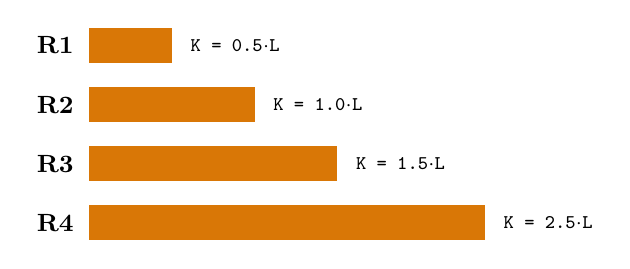
\begin{tikzpicture}[scale=0.75]
        \foreach[count=\i from 1] \rr/\kk/\ww in
            {1/0.5/1.4, 2/1.0/2.8, 3/1.5/4.2, 4/2.5/6.7} {
          \node[anchor=east, font=\small] at (-0.1, -\i + 0.35) {\textbf{R\rr}};
          \fill[orange] (0, -\i + 0.05) rectangle ++(\ww, 0.6);
          \node[anchor=west, font=\ttfamily\scriptsize] at (\ww + 0.15, -\i + 0.35)
            {K = \kk$\cdot$L};
        }
      \end{tikzpicture}
      \end{center}
      \vspace{0.4em}
      {\footnotesize Each round picks fresh seeds from the previous round's
        (sharper) distogram.}
    \end{column}

    \begin{column}{0.58\textwidth}
      \footnotesize\textbf{Pseudocode:}
      \begin{lstlisting}[style=code,basicstyle=\ttfamily\scriptsize\color{navy}]
distogram = naive_readout()

for K in [0.5L, 1.0L, 1.5L, 2.5L]:
    seeds = top-K contacts from
      distogram where p > 0.1,
      ordered long > medium > short

    prefix = <begin_statements>
             + [<{range}-range-contact>
                 <p_i> <p_j>
                for seed in seeds]

    distogram = readout under
                prefix, only for
                LDDT-shell pairs
      \end{lstlisting}
    \end{column}
  \end{columns}
  \vspace{0.5em}
  {\footnotesize
   \textbf{Contacts-only} --- distance-bin commits hurt LDDT (one-hot rows
   zero wrong-mode pairs).\quad
   {\color{green}\bfseries Standard expected-distance readout
   ($\sum p \cdot \text{midpoint}$) on the final distogram. No post-hoc
   sharpening.}}
\end{frame}

% --- Slide 6: progression ---
\newcommand{\progrow}[6]{%
  % args: y, label, value, bar-width, color, annotation
  \node[anchor=east, text=#5, font=\footnotesize\ttfamily,
        text width=4.6cm, align=right] at (4.35, #1) {#2};
  \fill[#5, opacity=0.6] (4.5, #1 - 0.17) rectangle ++(#4, 0.34);
  \node[anchor=west, text=#5, font=\footnotesize\ttfamily]
    at (4.5 + #4 + 0.1, #1) {#3};
  \node[anchor=west, text=#5, font=\scriptsize\itshape]
    at (4.5 + #4 + 1.05, #1) {#6};
}
\newcommand{\progrowH}[5]{%
  \node[anchor=east, text=#5, font=\footnotesize\bfseries\ttfamily,
        text width=4.6cm, align=right] at (4.35, #1) {#2};
  \fill[#5, opacity=0.95] (4.5, #1 - 0.17) rectangle ++(#4, 0.34);
  \node[anchor=west, text=#5, font=\footnotesize\bfseries\ttfamily]
    at (4.5 + #4 + 0.1, #1) {#3};
  \node[anchor=west, text=#5, font=\scriptsize\bfseries]
    at (4.5 + #4 + 1.05, #1) {$\leftarrow$ in-budget HEADLINE (+40.68\%)};
}
\begin{frame}{Progression: knob \textrightarrow{} knob \textrightarrow{} knob}
  \begin{center}
    \begin{tikzpicture}[scale=0.95]
      \progrow{0}{baseline\_naive}{0.2496}{2.66}{navy}{}
      \progrow{-0.55}{{+ sharpen (T=0.05)}}{0.2738}{2.92}{navy}{}
      \progrow{-1.10}{{seeded contacts (K=L, min=0.3)}}{0.2816}{3.00}{navy}{}
      \progrow{-1.65}{{iter R=3 (K=L, min=0.1)}}{0.3376}{3.60}{navy}{}
      \progrow{-2.20}{{iter R=3 grow [0.5, 1, 1.5]}}{0.3421}{3.65}{navy}{}
      \progrowH{-2.75}{{iter R=4 grow [0.5, 1, 1.5, 2.5]}}{0.3511}{3.74}{green}
      \progrow{-3.30}{{}}{0.3744}{3.99}{orange}{$\leftarrow$ +50\% bar (not cleared)}
      \progrow{-3.85}{GT-oracle (diagnostic only)}{0.7167}{7.64}{grey}{}
    \end{tikzpicture}
  \end{center}
  \vspace{0.4em}
  {\small\color{navy}+10\% bar (0.2746) cleared by sharpening alone.\
    +15.94\% by seeded + sharpen.}\\
  {\small\color{navy}Iteration with growing K is the big lever past +25\%.\
    \textbf{+40.68\% in 4373\,s (3.16$\times$ baseline, in budget).}}
\end{frame}

% --- Slide 7: per-protein chart ---
\begin{frame}{Per-protein results vs the +50\% bar}
  \begin{center}
    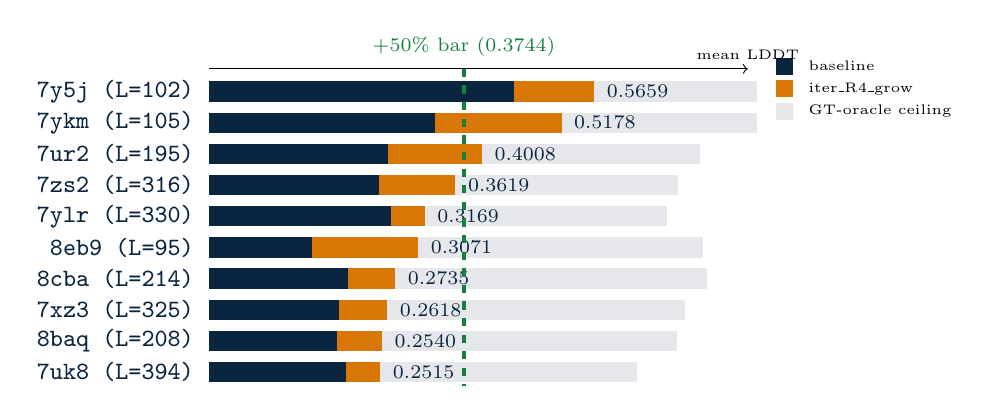
\begin{tikzpicture}[scale=0.72]
      % rows: protein, L, baseline, final, oracle
      \foreach[count=\i from 0] \name/\Len/\bv/\fv/\ov in {%
        7y5j/102/0.4485/0.5659/0.8044,
        7ykm/105/0.3317/0.5178/0.8052,
        7ur2/195/0.2633/0.4008/0.7219,
        7zs2/316/0.2500/0.3619/0.6895,
        7ylr/330/0.2673/0.3169/0.6734,
        8eb9/95/0.1510/0.3071/0.7254,
        8cba/214/0.2045/0.2735/0.7319,
        7xz3/325/0.1913/0.2618/0.6993,
        8baq/208/0.1872/0.2540/0.6870,
        7uk8/394/0.2010/0.2515/0.6290} {
        \pgfmathsetmacro\yp{-\i * 0.55}
        \node[anchor=east, text=navy, font=\small\ttfamily]
          at (-0.1, \yp) {\name\ (L=\Len)};
        \pgfmathsetmacro\wo{\ov * 12}
        \pgfmathsetmacro\wf{\fv * 12}
        \pgfmathsetmacro\wb{\bv * 12}
        \fill[lightgrey] (0, \yp - 0.18) rectangle ++(\wo, 0.36);
        \fill[orange] (0, \yp - 0.18) rectangle ++(\wf, 0.36);
        \fill[navy] (0, \yp - 0.18) rectangle ++(\wb, 0.36);
        \node[anchor=west, font=\scriptsize, text=navy]
          at (\wf + 0.05, \yp) {\fv};
      }
      % +50% bar
      \draw[green, line width=1.5pt, dashed]
        (4.493, 0.4) -- (4.493, -5.2);
      \node[anchor=south, font=\scriptsize, text=green]
        at (4.493, 0.45) {+50\% bar (0.3744)};
      % legend
      \fill[navy] (10, 0.3) rectangle ++(0.3, 0.3);
      \node[right, font=\tiny] at (10.4, 0.45) {baseline};
      \fill[orange] (10, -0.1) rectangle ++(0.3, 0.3);
      \node[right, font=\tiny] at (10.4, 0.05) {iter\_R4\_grow};
      \fill[lightgrey] (10, -0.5) rectangle ++(0.3, 0.3);
      \node[right, font=\tiny] at (10.4, -0.35) {GT-oracle ceiling};
      \draw[->, thin] (0, 0.4) -- (9.5, 0.4) node[above, font=\tiny] {mean LDDT};
    \end{tikzpicture}
  \end{center}
  \vspace{-0.5em}
  {\small\color{navy}\textbf{4 / 10 proteins pass the +50\% bar} on this single
    algorithm. The hard misses (8baq, 7uk8, 7xz3, 8cba, 8eb9, 7ylr) all have
    huge oracle headroom (0.43--0.55) --- model has the capacity, but its
    honest contact predictions remain sparse on these.}
\end{frame}

% --- Slide 8: what didn't work ---
\begin{frame}{What didn't work}
  \begin{itemize}
    \setlength\itemsep{0.4em}
    \item[\color{red}$\times$] \textbf{Sampled contact prefixes.}
      Model emits only 2--33 contacts before transitioning to
      \code{<distance>}; sampling-based seed selection has lower precision
      than top-K marginal. {\small\color{grey}\itshape
      +2.9\% single, +0.3\% M=5 average (averaging blurs distograms).}
    \item[\color{red}$\times$] \textbf{Distance-bin commits.}
      Inject \code{<distance> ... <d\_X.X>} statements for high-confidence pairs.
      Pair becomes one-hot row $\rightarrow$ LDDT zero when mode is wrong.
      {\small\color{grey}\itshape
      Net: 0.3503 vs 0.3511 (no change). Killed.}
    \item[\color{red}$\times$] \textbf{$K = 2L$ seeded contacts.}
      Lower-precision tail seeds poison the readout.
      {\small\color{grey}\itshape $-1.2\%$ vs $K = L$.
        Precision $>$ count.}
    \item[\color{red}$\times$] \textbf{Mixture-of-distograms / per-pair max-confidence.}
      Variants aren't differently wrong --- just less wrong, same direction.
      {\small\color{grey}\itshape Worse than the best single algorithm.}
    \item[\color{red}$\times$] \textbf{Sharpening on top of iter\_R4\_grow.}
      \code{p' = softmax(log p / T)}. T=1.0 (no sharpen) wins.
      {\small\color{grey}\itshape Sharpening only helps when distributions are
      high-entropy from bad context. Matches the GT-oracle pattern.}
  \end{itemize}
\end{frame}

% --- Slide 9: takeaways ---
\begin{frame}{Takeaways}
  \small
  \begin{itemize}
    \setlength\itemsep{0.25em}
    \item[\color{navy}\textbullet] \textbf{Context $>$ sampling.}
      Top-K from the marginal contact distribution beats sampling contact
      statements autoregressively at any $T$.
    \item[\color{navy}\textbullet] \textbf{Iteration enriches the high-confidence
      contact pool.} Contacts above 0.5 prob grow 5--75$\times$ after 3
      iterations. Later rounds can afford larger $K$ without losing precision.
    \item[\color{navy}\textbullet] \textbf{Growing $K$ matters.}
      Cautious early ($K=0.5L$), bold late ($K=2.5L$) beats fixed $K=L$ or
      $K=2L$. Round 1's noisy bold picks would limit later rounds.
    \item[\color{navy}\textbullet] \textbf{Precision $>$ count.}
      $K=2L$ always hurts. Distance commits hurt. What works is exactly the
      model's most-confident predictions, nothing extra.
    \item[\color{navy}\textbullet] \textbf{Sharpening rescues bad context, not
      good context.} Big gain on naive (+9.7\%); zero gain on oracle.
    \item[\color{navy}\textbullet] \textbf{Contact prediction is the
      bottleneck, not the model.} GT-oracle reaches 0.72. For hard proteins,
      the model just doesn't honestly identify enough contacts at inference time.
  \end{itemize}
\end{frame}

% --- Slide 10: reproducer ---
\begin{frame}[fragile]{Reproducer}
  {\footnotesize 10 proteins \textperiodcentered\ A100 40\,GB \textperiodcentered\ bf16
    \textperiodcentered\ vLLM 0.7.3 \textperiodcentered\
    $\sim$4373\,s wall (3.16$\times$ baseline)}\\[0.3em]
  \begin{lstlisting}[style=code,basicstyle=\ttfamily\footnotesize\color{navy}]
# 1. Produce the baseline full-distogram prior
uv run python run_baseline.py --dtype bfloat16 --n-gpus 1
uv run python snapshot_distograms.py --to distogram_baseline_naive.npz

# 2. Run iter_R4_grow_05_10_15_25
uv run python run_iterative.py --dtype bfloat16 --n-gpus 1 \
    --algorithm iter_R4_grow_05_10_15_25 \
    --n-rounds 4 \
    --k-contacts-per-L-per-round 0.5 1.0 1.5 2.5 \
    --k-distances-per-L-per-round 0.0 0.0 0.0 0.0 \
    --min-contact-prob 0.1 \
    --prior-name distogram_baseline_naive.npz

# Result: mean LDDT 0.3511 (+40.68% over baseline 0.2496)
  \end{lstlisting}
  \vspace{0.2em}
  {\scriptsize\color{grey}\ttfamily Branch: exp/27-improved-inference-algorithm \
    \textperiodcentered\ \ Narrative + rows: RESULTS\_LOG.md, data/experiments.tsv}
\end{frame}

\end{document}
